% We define .... 
Let $\mathcal{W}\subset \mathbb{R}^2$ be a 
% compact (i.e., closed and bounded) 
polygonal workspace, which may contain one or multiple connected components. 
A {\em critical subset} of $\mathcal{W}$ needs to be guarded by $k$ 
%\sw{jumpping from $r_i$ to inditinguishable}
indistinguishable point guards with range sensing capabilities. For 
example, the workspace may be a forest reserve and the critical subset 
may be its boundary. Or, the workspace may be a high-security facility, 
e.g., a prison, and the critical subset the prison yard. The $i$th 
guard, $1\le i\le k$, located at $c_i \in \mathbb{R}^2$, can monitor a circular 
area of radius $r_i$ centered at $c_i$ with $r_i$ being a variable. For 
example, the guard may be a watchtower equipped with a vision sensor 
that can detect intruders. As the watchtower's altitude increases, 
its sensing range also increases; but its monitoring quality will 
decrease at the same time due to resolution loss. In this study, we seek 
to compute the optimal strategy to deploy these $k$ guards so that the 
required sensing range, $\max_i r_i$, could be minimized. 

More formally, we model a connected component of $\W$ as some 2D polygonal region
containing zero or more simple polygonal obstacles. 
For a bounded set $D \subset \mathbb{R}^2$, we define
\begin{equation*}
size(k, D) = \min_{c_1, \dots, c_k\in \mathbb{R}^2}\ \max_{p\in D}\ \min_{1\leq i\leq k} \lVert c_i - p \rVert_2 
\end{equation*}
and use $B(c, r)$ to denote the disc of radius $r$ centered at a point $c 
\in \mathbb{R}^2$ (the definition of $size(k, D)$ is used extensively in later 
sections). 
Intuitively, $size(k,D)$ represents the minimum radius needed such that there
exisits $k$ circles with radius $size(k, D)$ that can cover the 2D bounded region $D$ entirely.
% The critical subset of interest in this work is either part of the boundary of $\W$, denoted $\partial \W$, or $\W$ itself. 
The main problem studied in this work is:

\begin{problem}[Optimal Set Guarding with 2D Sensors]
Given a polygonal workspace $\W \subset \mathbb{R}^2$, let $D \subset \W$ be a 
critical subset to be guarded by $k$ robots each with a variable coverage radius of $r$. Find 
the smallest $r$ and corresponding robot locations $c_1, \dots, c_k\in \mathbb{R}^2$, such that $D \subset \cup_i B(c_i, r)$.
\end{problem}

For making accurate statements about computational complexity, we make
the assumption that the length of $\partial \W$ is bounded by a polynomial with respect 
to the complexity of $\W$, (i.e. the number of vertices of the polygon). 
% Furthermore, we assume the possible 
% sensing radius of the robots is lower and upper bounded by some constants, 
% as is the case in practice. 

For convenience, we give specific names to these optimal guarding 
problems based critical subset types. If the critical 
subset belongs to $\partial \W$, we denote the problem as {\em optimal 
perimeter guarding with 2D sensors} or \opgt. If the critical subset 
is $\W$, we denote the problem as {\em optimal region guarding with 
2D sensors} or \orgt. When there is no need to distinguish, the problem 
is denoted as {\em optimal set guarding with 2D sensors} (\osgt). 
%The decision versions of \opgt and \orgt are denoted 
%\dopgt and \dorgt, respectively. 

As an example, to guard the boundary of a plus-shaped polygon with $5$ 
robots, an optimal solution could be ~\ref{fig:osg-example} where the 
inner circle covers $4$ disconnected boundary segments, such pattern 
in the optimal solution also renders \opgt much more difficult than 
the simplified 1D sensing model studied in \cite{fenghangaoyu2019efficient} 
(indeed, \opgt becomes hard to approximate, as will be shown shortly). 
The solution is also optimal under the \orgt formulation.
\begin{figure}[ht]
    \centering
		\vspace*{3mm}
    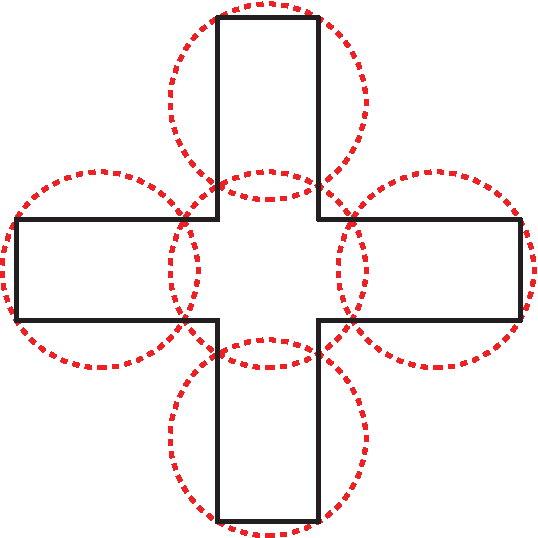
\includegraphics[scale=0.35]{chapters/osg/figures/exp_fig-e-eps-converted-to.pdf}
		\vspace*{1.5mm}
    \caption{An example showing an optimal solution of using five discs
		to cover the plus-shaped polygon. The solution is optimal for both 
		\opgt and \orgt formulations.}
    \label{fig:osg-example}
\end{figure}

